\section{初识神经网络}
\label{sec:chapter7}

\subsection{神经元模型}

\begin{figure}[H]
    \centering
    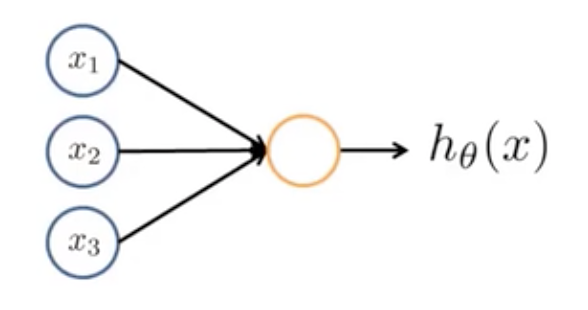
\includegraphics[width=0.4\linewidth]{figs/Chap_7_neuron.png}
    \vspace{-2ex}
\end{figure}

神经元可以视为一个函数：它接收上一层节点的输出，将各输入按权重组合，再经过激活函数得到新的输出，即：
\[
h_\theta(x)=f(\theta, x)
\]
这里 $\theta=(\theta_0,\theta_1,\cdots,\theta_n)^T,\,x=(x_0,x_1,\cdots,x_n)^T$.

\begin{note}
上图省略了 $x_0\equiv 1$ 这一偏置项。
\end{note}

神经元输出 $h_\theta(x)$ 由激活函数计算。激活函数为神经网络引入非线性，使多层网络能够表示比单纯线性变换更复杂的关系。此处采用 $\text{sigmoid}$ 函数，即 $h_\theta(x)=g(\theta^Tx)=\frac{1}{1+e^{-\theta^Tx}}$. 


\subsection{神经网络}

\begin{figure}[H]
    \centering
    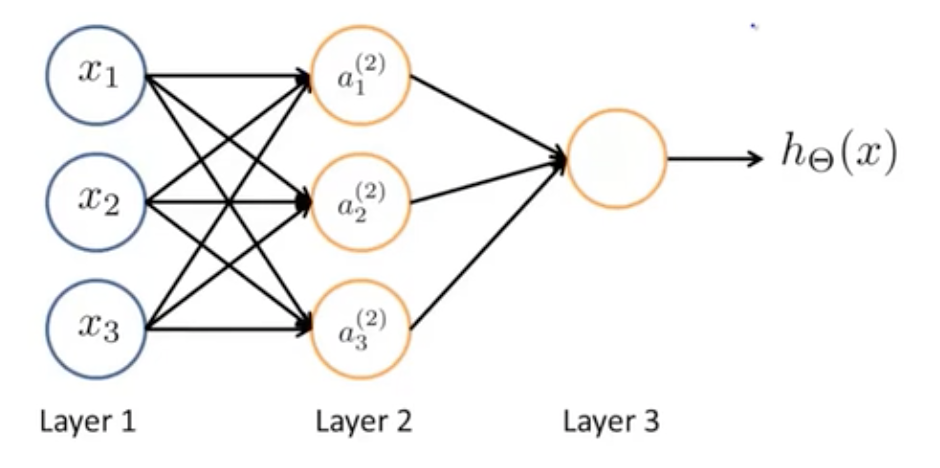
\includegraphics[width=0.5\linewidth]{figs/Chap_7_neuron_network.png}
    \vspace{-2ex}
\end{figure}

神经网络由多层相互连接的神经元组成。第一层称为输入层，负责接收原始特征；最后一层称为输出层，给出模型的预测；位于二者之间的各层称为隐藏层。信息从输入层开始，逐层计算并传递到输出层，这一过程称为前向传播。

\begin{note}
上图同样省略了 $x_0(a_0^{(1)})\equiv a_0^{(2)}\equiv1$ 偏置项。
\end{note}

下面单独分析第 $i$ 层到第 $i+1$ 层的传播过程。设 $s_i$ 为第 $i$ 层的神经元数量（\textbf{不包含偏置项}），则第 $i+1$ 层的每个神经元都与一组独立参数对应。对于第 $k$ 个神经元，其参数记为 $\theta^{(i)}_k$，并满足 $a^{(i+1)}_k=h_{\theta^{(i)}_k}(\hat a^{(i)})=g\left({\theta_k^{(i)}}^T\hat a^{(i)}\right)$. 其中，$\hat a^{(i)}\in\mathbb R^{s_i+1}$ 表示在 $a^{(i)}$ 前加入偏置项后的向量。将下一层所有神经元的计算合并，即可写成矩阵形式：
\[
a^{(i+1)}=g\left(\Theta^{(i)}\hat a^{(i)}\right)
\]
其中，$\Theta^{(i)}\in\mathbb R^{s_{i+1}\times(s_i+1)}$. 

\begin{note}
也可以将偏置项对应的参数向量 $b$ 单独列出，将上式写为：
\[
a^{(i+1)}=g\left(\Theta^{(i)}a^{(i)}+b^{(i)}\right)
\]
其中，$\Theta^{(i)}\in\mathbb R^{s_{i+1}\times s_i},\,b\in\mathbb R^{s_{i+1}}$. 本文仍沿用前一种写法。
\end{note}


\subsection{神经网络实现门电路}

下面通过门电路示例直观说明神经网络参数如何控制输出。

考虑一个输入层有 $2$ 个神经元（不包括偏置项）且取值 $\in\{0,1\}$、输出层有 $1$ 个神经元且取值 $\in\{0,1\}$ 的神经网络。如果我们将其参数设置为：$\Theta^{(1)}=(-30,20,20)^T$，那么我们有：

\begin{table}[H]
    \centering
    \begin{tabularx}{0.4\linewidth}{cYc}
      \toprule
      输入 1 & 输入 2 & 输出 \\
      \midrule
      0 & 0 & $g(-30)\approx 0$ \\
      0 & 1 & $g(-10)\approx 0$ \\
      1 & 0 & $g(-10)\approx 0$ \\
      1 & 1 & $g(10)\approx 1$  \\
      \bottomrule
    \end{tabularx}
\end{table}

从表中可以看出，只有两个输入同时为 $1$ 时，线性组合才为正且输出接近 $1$；其他情况下输出均接近 $0$. 因此，这个神经元实现了与门。

通过选择不同参数，同样可以实现或门和非门。进一步将这些基本门组合起来，多层神经网络还可以表示单个线性分类器无法直接实现的异或门、同或门等逻辑电路。这也说明隐藏层能够逐层组合较简单的特征，形成更复杂的决策规则。


\subsection{代码实现}

本节仍以手写数字识别为例，但暂不训练参数。参数 $\Theta$ 已在 \texttt{ex3weights.mat} 中给出，只需按照神经网络结构逐层执行前向传播。

\begin{lstlisting}[language=Python]
import numpy as np
from scipy.io import loadmat
import matplotlib.pyplot as plt
import matplotlib

m = 5000
n = 401

data = loadmat('ex3data1.mat')
X = data['X'] # (5000, 400)
X = np.hstack((np.ones((m, 1)), X)) # (5000, 401)
y = data['y'] # (5000, 1)

data = loadmat('ex3weights.mat')
Theta1 = data['Theta1'] # (25, 401)
Theta2 = data['Theta2'] # (10, 26)

def sigmoid(z):
	return 1 / (1 + np.exp(-z))

def predict(x):
	"""
	x: (401, )
	"""
	a1 = x.reshape((401, 1))
	a2 = np.matmul(Theta1, a1)
	a2 = sigmoid(a2) # (25, 1)
	a2 = np.vstack((np.ones((1, 1)), a2)) # (26, 1)
	a3 = np.matmul(Theta2, a2)
	a3 = sigmoid(a3)
	return a3.argmax(axis=0)[0] + 1

Sum = np.zeros(11)
Hit = np.zeros(11)
Accuracy = np.zeros(11)
hit = 0
for id in range(5000):
	Sum[y[id][0]] += 1
	if predict(X[id, :].T) == y[id][0]:
		Hit[y[id][0]] += 1
		hit += 1
for i in range(1, 11):
	Accuracy[i] = Hit[i] / Sum[i]
	print(str(i)+":", str(Accuracy[i] * 100)+"%")
print("tot:", str(hit / 5000 * 100)+"%")
\end{lstlisting}

各数字及整体的准确率如下：

\begin{table}[H]
    \centering
    \small
    \begin{tabularx}{\linewidth}{lYYYYYYYYYYY}
    \toprule
    数字 & 1 & 2 & 3 & 4 & 5 & 6 & 7 & 8 & 9 & 0 & Total \\
    \midrule
    准确率 & 98.2\% & 97.0\% & 96.0\% & 96.8\% & 98.4\% & 98.6\% & 97.0\% & 98.2\% & 95.8\% & 99.2\% & 97.5\% \\
    \bottomrule
    \end{tabularx}
\end{table}

注意：训练集准确率并不能作为模型评估结果。
